\newpage
\section*{\LARGE{Глава 2. Метод поиска кратчайшего пути}}
\addcontentsline{toc}{section}{Глава 2.  Метод поиска кратчайшего пути}
\hskip 12 mm
Существуют различные подходы для поиска оптимального пути между двумя объектами. Одним из способов решения данной задачи является её сведение к поиску кратчайшего пути на графе. Для этого требуется взять определенный набор точек $P$, лежащих в области построения $Q$, на их основе сгенерировать вычислительную сетку, которую можно преобразовать в граф. Каждое ребро получившегося графа является прямым отрезком, принадлежащим области $Q$, соответственно, его вес можно вычислять, как интегральную сумму, определение которой было дано в гл. 1. После того как граф построен, можно пользоваться методами поиска кратчайшего пути.
\par
Главным плюсом данного подхода является отсутствие локальных минимумов и то, что для каждого построенного графа найденный путь между точками будет являться кратчайшим. И не возникает такой проблемы, как обход области с высокой стоимостью строительства.  
\begin{figure}[H]
	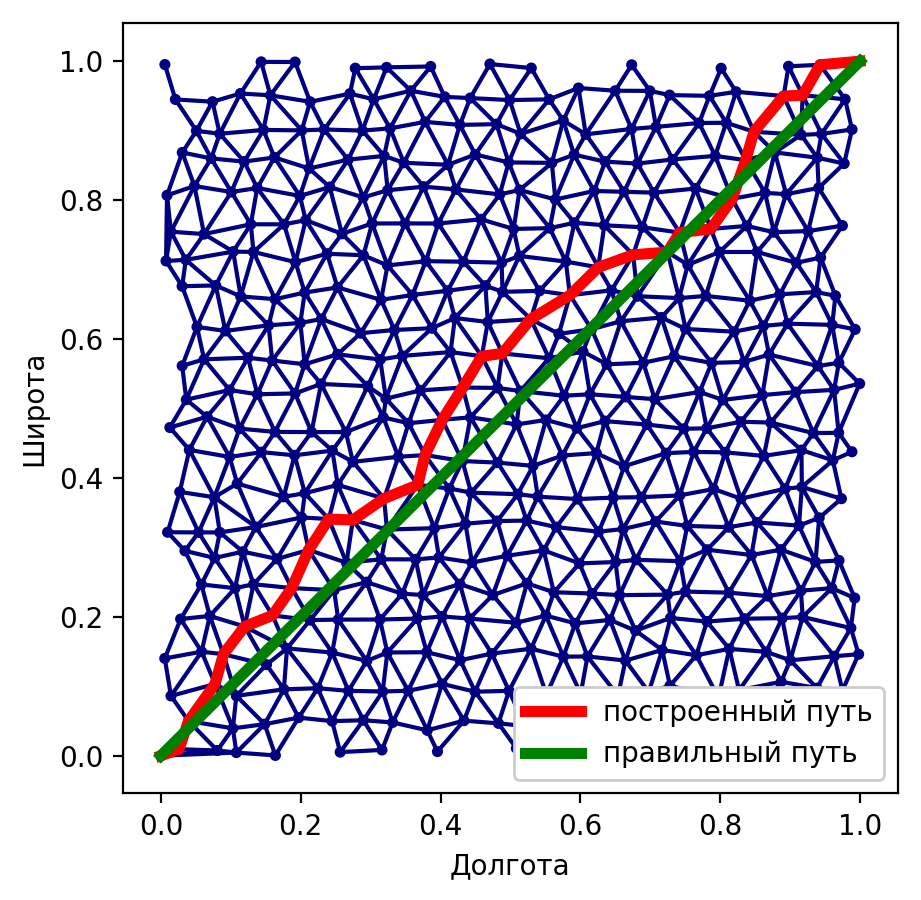
\includegraphics[width=0.5\textwidth]{images/2_2.png}
	\caption{Поиск пути на графе}
	\label{pic:graph_path}
\end{figure}
\vskip 4mm
\par
Однако данный подход не лишен недостатков. Самая большая проблема --- это точность получаемого решения, что можно увидеть на рис. \ref{pic:graph_path}. Оптимальный путь представляет собой прямую линию соединяющую два противоположных угла квадрата, а путь, найденный на графе, представляет собой ломаную линию, лежащую, хоть и недалеко от оптимального решения, но и не совпадающего с ним. Поэтому остро стоит проблема поиска правильного метода генерации вычислительной сетки.
\par 
Существуют различные алгоритмы поиска кратчайшего пути на графе. Так как нашей задачей является нахождение пути с минимальной стоимостью между парой вершин без учета различного рода ограничений на число рёбер в построенном пути, было решено использовать алгоритм А* \cite{A_star}. Основным его преимуществом является наличие эвристической функции, значительно уменьшающей время поиска пути. Только в случае нашей задачи поиск оптимальной эвристической функции для оценки расстояния между двумя вершинами нетривиален, в связи с неоднородностью стоимостной функции $c$ и функцией высоты рельефа $h$.
\par
Также решение, полученное на графе, является хорошим начальным приближением для дальнейшего расчёта, используя методы оптимизации.
